\section{Implementation}

\begin{figure}[H]
    \centering
    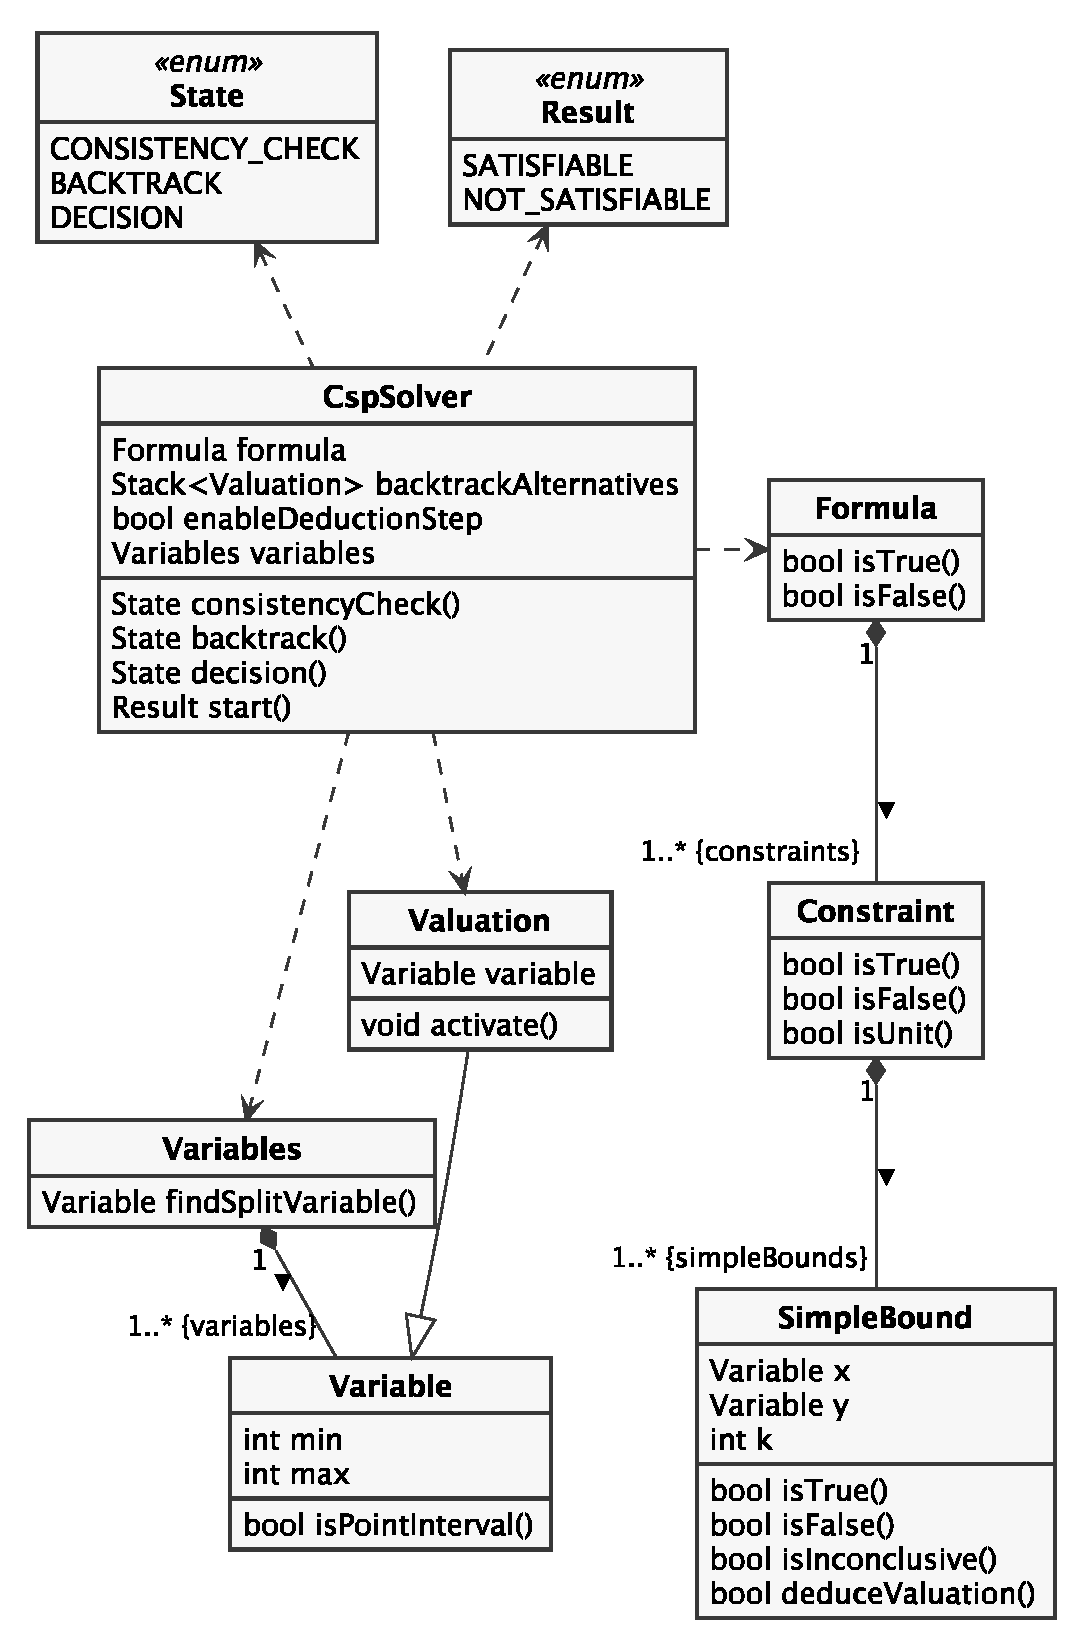
\includegraphics[width=.6\textwidth]{images/class-diagram}
    \caption{UML class diagram of our implementation of algorithm $\mathcal{A}$.}
    \label{fig:class-diagram}
\end{figure}


\subsection{Algorithms $\mathcal{A}$ and $\mathcal{B}$}

\paragraph{}
Fig.~\ref{fig:class-diagram} shows an UML class diagram of the implementation.
The class \texttt{Formula} models CSP formulae of the type $F = c_1 \wedge c_2 \wedge ... \wedge c_n$, with $c_i \in C$.
It defines a member \texttt{java.util.ArrayList} over \texttt{Constraint}.
The classes \texttt{Constraint} and \texttt{SimpleBound} model simple constraints and simple bounds, respectively, as defined in def.~2 from~\cite{MF19}.
\texttt{Constraint}, too, defines a \texttt{java.util.ArrayList} member, except this one is over \texttt{SimpleBound}.
The methods \texttt{isTrue()}, \texttt{isFalse()} and \texttt{isInconclusive()} of these classes can be used to compute the truth values of the respective instance.
The class \texttt{Variable} models a variable, with a lower and an upper bound; \texttt{Valuation} models an interval valuation of a single variable.
Our implementation's use of valuations is described in section~\ref{ssec:valuations}.

\paragraph{}
The main part is the class \texttt{CspSolver}.
It implements the algorithm $\mathcal{A}$, and, by enabling the flag \texttt{CspSolver.enableDeductionStep}, also algorithm $\mathcal{B}$. This implementation is a plain implementation of the algorithms described in~\cite{MF19}, without any optimisations.

After assigning an instance of \texttt{Formula}, the method \texttt{CspSolver.start()} can be called.
Inside that method runs a very simple state machine, realised by an infinite loop and the states in the enumeration \texttt{State}.
Following the algorithm, the initial state is \texttt{State.CONSISTENCY\_CHECK}.
Depending on the state, the corresponding method of \texttt{CspSolver} is called, where each method returns the next state.

As one would expect, the method \texttt{CspSolver.consistencyCheck()} implements step 1, \texttt{.backtrack()} step 2 and \texttt{.decision()} step 3 of algorithms $\mathcal{A}$ and $\mathcal{B}$ (the latter after enabling the flag \texttt{CspSolver.enableDeductionStep}).

\texttt{CspSolver.backtrack()} and \texttt{.decision()} use the \texttt{backtrackAlternatives} member of the same class to store the backtrack alternatives.
It's an instance of the \texttt{java.util.Stack} class from the Java standard library.
It offers everything our implementation needed, so we didn't see any reason to create our own stack implementation.

When the algorithm reaches a result in either \texttt{CspSolver.consistencyCheck()} or \texttt{.backtrack()}, a special case of \texttt{State} is returned by these methods (not seen in figure~\ref{fig:class-diagram}).
This is converted to an instance of \texttt{Result} and returned by \texttt{CspSolver.start()}, thus exiting the infinite loop.


\subsubsection{Interval Valuations}\label{ssec:valuations}

\paragraph{}
Instead of having a single data structure to store the interval valuations of all variables (like the function $\rho$ from the task description indicates), a new instance of \texttt{Valuation} is created every time a new interval valuation is needed (simply ``valuations'' from now on).

\todo[inline]{Groesser machen?}

\begin{multicols}{2}

\begin{figure}[H]
  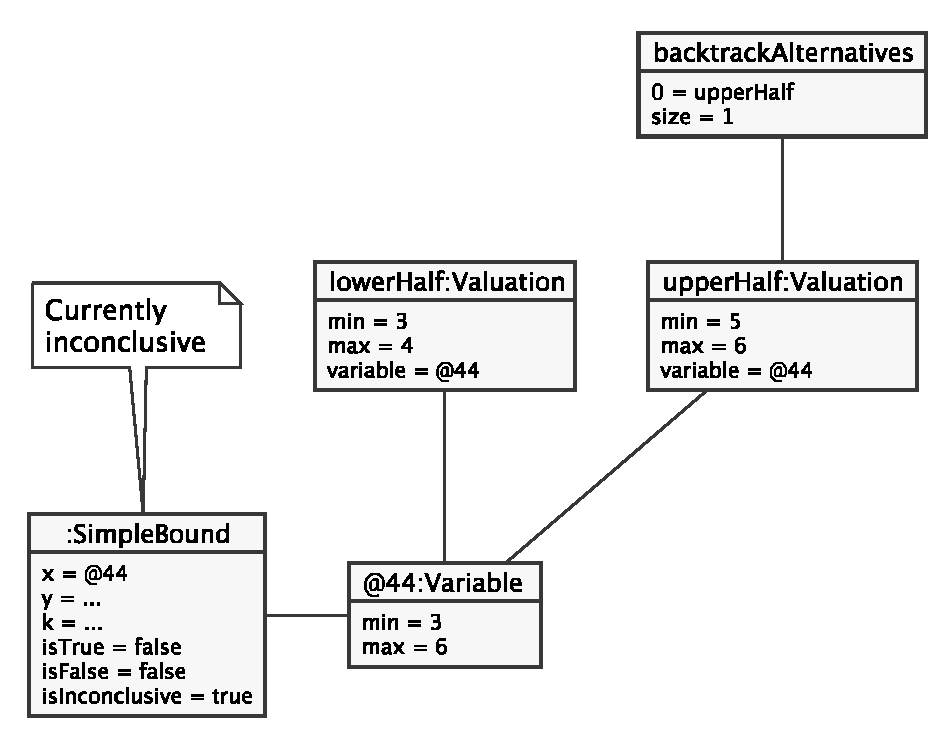
\includegraphics[width=.5\textwidth]{images/valuation-before}
  \caption{UML object diagram \textbf{before} calling \texttt{lowerHalf.activate()} in line 145 of \texttt{CspSolver.java}.}
  \label{fig:valuation-before}
\end{figure}

\columnbreak    

\begin{figure}[H]
  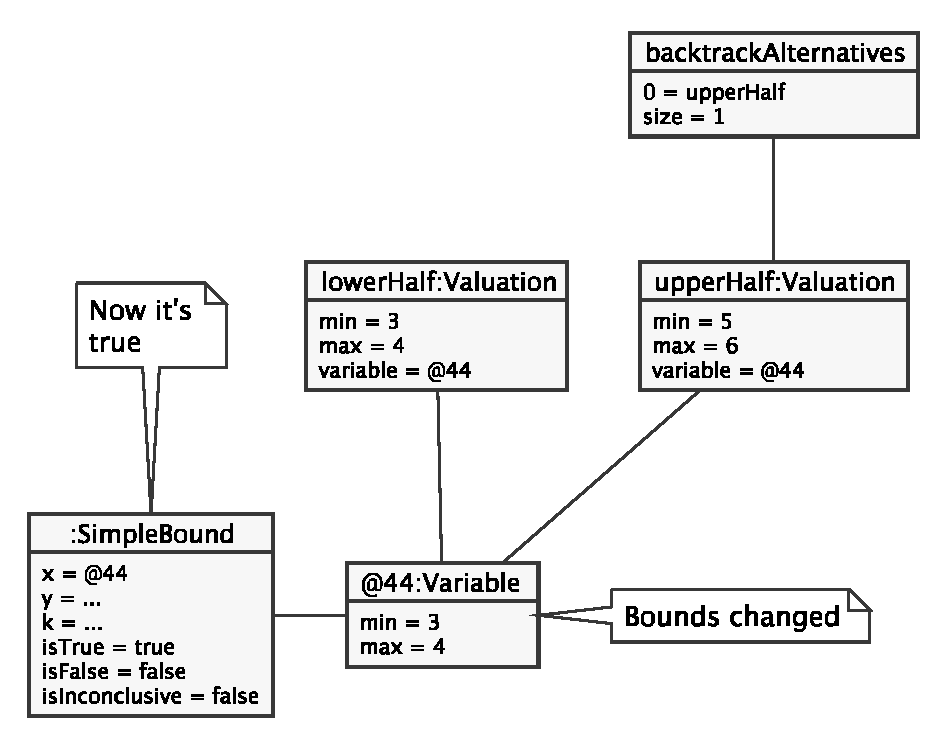
\includegraphics[width=.5\textwidth]{images/valuation-after}
  \caption{UML object diagram \textbf{after} calling \texttt{lowerHalf.activate()} in line 145 of \texttt{CspSolver.java}.}
  \label{fig:valuation-after}
\end{figure}

\end{multicols}


\paragraph{}
Valuations utilise Java's reference semantic to alter the lower and upper bounds of variables they are intended for.
Just as simple bounds, valuations store only references to the actual variables.
So when a valuation changes the bounds of the variable stored inside it, the bounds of the same variable stored inside some \texttt{SimpleBound}-instance is also changed (because they're technically the same).
The next time the truth value of one of those simple bounds is computed, the new bounds are used.
\texttt{Valuation.activate()} can be used to assign new bounds to the \texttt{Variable} instance stored inside that valuation.
The object diagrams seen in fig.~\ref{fig:valuation-before} and fig.~\ref{fig:valuation-after} show what happens in memory when a valuation is activated.

Because the algorithm doesn't use valuations more than once, they are only stored in the backtrack alternatives stack, if at all.
When two new valuations are created during the decision step, the one not stored as a backtrack alternative is directly activated and then left to be collected by the JVM's garbage collector.
During the backtrack step, the alternative is popped off of the \texttt{CspSolver.backtrackAlternatives}-stack, and then similarly activated and left to be collected.


\subsubsection{Implementation of Algorithm $\mathcal{B}$}

\paragraph{}
As described before, our implementation allows to switch to algorithm~$\mathcal{B}$ by enabling the flag \texttt{CspSolver.enableDeductionStep}.
If that flag is enabled, the consistency check changes its behaviour when there're no false constraints and not all constraints are true.
In that case, the implementation iterates over all constraints, uses \texttt{Constraint.isUnit()} to check whether its unit and, if so, calls \texttt{SimpleBound.deduceValuation()} on all simple bounds of that constraint to try to deduce new valuations for $x$ and $y$ of that simple bound as defined in algorithm~$\mathcal{B}$.

If at least one variable's valuation could be narrowed down by doing this, the method returns true.
In that case, the implementation switches to the state \texttt{State.CONSISTENCY\_CHECK}, otherwise to \texttt{State.DECISION}.


\subsubsection{Lazy Clause Evaluation \& Decision Heuristics}

\paragraph{}
\todo[inline]{Grob skizzieren}
